
\definecolor{cebebeb}{RGB}{235,235,235}
\definecolor{c333333}{RGB}{51,51,51}
\definecolor{c4d4d4d}{RGB}{77,77,77}


\def \globalscale {1.000000}
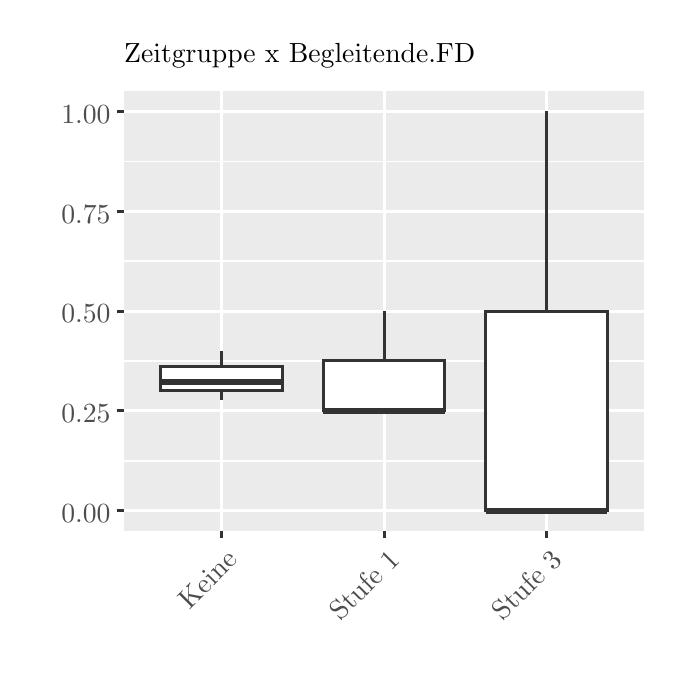
\begin{tikzpicture}[y=1mm, x=1mm, yscale=\globalscale,xscale=\globalscale, every node/.append style={scale=\globalscale}, inner sep=0pt, outer sep=0pt]
  \path[fill=white,line cap=round,line join=round,miter limit=10.0] ;



  \path[draw=white,fill=white,line cap=round,line join=round,line 
  width=0.38mm,miter limit=10.0] (0.0, 80.0) rectangle (80.0, 0.0);



  \path[fill=cebebeb,line cap=round,line join=round,line width=0.38mm,miter 
  limit=10.0] (12.07, 72.09) rectangle (78.07, 16.31);



  \path[draw=white,line cap=butt,line join=round,line width=0.19mm,miter 
  limit=10.0] (12.07, 25.18) -- (78.07, 25.18);



  \path[draw=white,line cap=butt,line join=round,line width=0.19mm,miter 
  limit=10.0] (12.07, 37.86) -- (78.07, 37.86);



  \path[draw=white,line cap=butt,line join=round,line width=0.19mm,miter 
  limit=10.0] (12.07, 50.54) -- (78.07, 50.54);



  \path[draw=white,line cap=butt,line join=round,line width=0.19mm,miter 
  limit=10.0] (12.07, 63.22) -- (78.07, 63.22);



  \path[draw=white,line cap=butt,line join=round,line width=0.38mm,miter 
  limit=10.0] (12.07, 18.85) -- (78.07, 18.85);



  \path[draw=white,line cap=butt,line join=round,line width=0.38mm,miter 
  limit=10.0] (12.07, 31.52) -- (78.07, 31.52);



  \path[draw=white,line cap=butt,line join=round,line width=0.38mm,miter 
  limit=10.0] (12.07, 44.2) -- (78.07, 44.2);



  \path[draw=white,line cap=butt,line join=round,line width=0.38mm,miter 
  limit=10.0] (12.07, 56.88) -- (78.07, 56.88);



  \path[draw=white,line cap=butt,line join=round,line width=0.38mm,miter 
  limit=10.0] (12.07, 69.56) -- (78.07, 69.56);



  \path[draw=white,line cap=butt,line join=round,line width=0.38mm,miter 
  limit=10.0] (24.44, 16.31) -- (24.44, 72.09);



  \path[draw=white,line cap=butt,line join=round,line width=0.38mm,miter 
  limit=10.0] (45.07, 16.31) -- (45.07, 72.09);



  \path[draw=white,line cap=butt,line join=round,line width=0.38mm,miter 
  limit=10.0] (65.69, 16.31) -- (65.69, 72.09);



  \path[draw=c333333,line cap=butt,line join=round,line width=0.38mm,miter 
  limit=10.0] (24.44, 37.18) -- (24.44, 39.13);



  \path[draw=c333333,line cap=butt,line join=round,line width=0.38mm,miter 
  limit=10.0] (24.44, 34.06) -- (24.44, 32.89);



  \path[draw=c333333,fill=white,line cap=butt,line join=miter,line 
  width=0.38mm,miter limit=10.0] (16.71, 37.18) -- (16.71, 34.06) -- (32.18, 
  34.06) -- (32.18, 37.18) -- (16.71, 37.18) -- (16.71, 37.18)-- cycle;



  \path[draw=c333333,line cap=butt,line join=miter,line width=0.75mm,miter 
  limit=10.0] (16.71, 35.23) -- (32.18, 35.23);



  \path[draw=c333333,line cap=butt,line join=round,line width=0.38mm,miter 
  limit=10.0] (45.07, 37.86) -- (45.07, 44.2);



  \path[draw=c333333,line cap=butt,line join=round,line width=0.38mm,miter 
  limit=10.0] ;



  \path[draw=c333333,fill=white,line cap=butt,line join=miter,line 
  width=0.38mm,miter limit=10.0] (37.33, 37.86) -- (37.33, 31.52) -- (52.8, 
  31.52) -- (52.8, 37.86) -- (37.33, 37.86) -- (37.33, 37.86)-- cycle;



  \path[draw=c333333,line cap=butt,line join=miter,line width=0.75mm,miter 
  limit=10.0] (37.33, 31.52) -- (52.8, 31.52);



  \path[draw=c333333,line cap=butt,line join=round,line width=0.38mm,miter 
  limit=10.0] (65.69, 44.2) -- (65.69, 69.56);



  \path[draw=c333333,line cap=butt,line join=round,line width=0.38mm,miter 
  limit=10.0] ;



  \path[draw=c333333,fill=white,line cap=butt,line join=miter,line 
  width=0.38mm,miter limit=10.0] (57.96, 44.2) -- (57.96, 18.85) -- (73.43, 
  18.85) -- (73.43, 44.2) -- (57.96, 44.2) -- (57.96, 44.2)-- cycle;



  \path[draw=c333333,line cap=butt,line join=miter,line width=0.75mm,miter 
  limit=10.0] (57.96, 18.85) -- (73.43, 18.85);



  \node[text=c4d4d4d,anchor=south east] (text811) at (10.33, 17.33){0.00};



  \node[text=c4d4d4d,anchor=south east] (text3063) at (10.33, 30.01){0.25};



  \node[text=c4d4d4d,anchor=south east] (text789) at (10.33, 42.69){0.50};



  \node[text=c4d4d4d,anchor=south east] (text423) at (10.33, 55.37){0.75};



  \node[text=c4d4d4d,anchor=south east] (text7751) at (10.33, 68.05){1.00};



  \path[draw=c333333,line cap=butt,line join=round,line width=0.38mm,miter 
  limit=10.0] (11.1, 18.85) -- (12.07, 18.85);



  \path[draw=c333333,line cap=butt,line join=round,line width=0.38mm,miter 
  limit=10.0] (11.1, 31.52) -- (12.07, 31.52);



  \path[draw=c333333,line cap=butt,line join=round,line width=0.38mm,miter 
  limit=10.0] (11.1, 44.2) -- (12.07, 44.2);



  \path[draw=c333333,line cap=butt,line join=round,line width=0.38mm,miter 
  limit=10.0] (11.1, 56.88) -- (12.07, 56.88);



  \path[draw=c333333,line cap=butt,line join=round,line width=0.38mm,miter 
  limit=10.0] (11.1, 69.56) -- (12.07, 69.56);



  \path[draw=c333333,line cap=butt,line join=round,line width=0.38mm,miter 
  limit=10.0] (24.44, 15.34) -- (24.44, 16.31);



  \path[draw=c333333,line cap=butt,line join=round,line width=0.38mm,miter 
  limit=10.0] (45.07, 15.34) -- (45.07, 16.31);



  \path[draw=c333333,line cap=butt,line join=round,line width=0.38mm,miter 
  limit=10.0] (65.69, 15.34) -- (65.69, 16.31);



  \node[text=c4d4d4d,anchor=south east,cm={ 0.71,0.71,-0.71,0.71,(26.58, 
  -67.57)}] (text3911) at (0.0, 80.0){Keine};



  \node[text=c4d4d4d,anchor=south east,cm={ 0.71,0.71,-0.71,0.71,(47.21, 
  -67.57)}] (text106) at (0.0, 80.0){Stufe 1};



  \node[text=c4d4d4d,anchor=south east,cm={ 0.71,0.71,-0.71,0.71,(67.83, 
  -67.57)}] (text4309) at (0.0, 80.0){Stufe 3};



  \node[anchor=south west] (text2860) at (12.07, 75.04){Zeitgruppe x 
  Begleitende.FD};




\end{tikzpicture}
